\newif\ifshowsolutions
%\showsolutionstrue
\documentclass{article}
\usepackage{listings}
\usepackage{amsmath}
\usepackage{subfig}
\usepackage{amsthm}
\usepackage{amsmath}
\usepackage{amssymb}
\usepackage{graphicx}
\usepackage{mdwlist}
\usepackage{geometry}
\usepackage{titlesec}
\usepackage{palatino}
\usepackage{mathrsfs}
\usepackage{fancyhdr}
\usepackage{paralist}
\usepackage{todonotes}
\usepackage{tikz}
\usepackage{float} % Place figures where you ACTUALLY want it
\usepackage{comment} % A hack to toggle sections
\usepackage{ifthen}
\usepackage{mdframed}
\usepackage{verbatim}
\usepackage{listings}
\usepackage{bbm}
\usepackage{upquote} % Prevents backticks replacing single-quotes in verbatim
\usepackage[strings]{underscore}
\usepackage[colorlinks=true]{hyperref}
\usetikzlibrary{positioning,shapes,backgrounds}

\geometry{margin=1in}
\geometry{headheight=2in}
\geometry{top=2in}

\setlength{\marginparwidth}{2.15cm}
\setlength{\parindent}{0em}
\setlength{\parskip}{0.6\baselineskip}

\rhead{}
\lhead{}

% Spacing settings.
\titlespacing\section{0pt}{12pt plus 2pt minus 2pt}{0pt plus 2pt minus 2pt}
\titlespacing\subsection{0pt}{12pt plus 4pt minus 2pt}{0pt plus 2pt minus 2pt}
\titlespacing\subsubsection{0pt}{12pt plus 4pt minus 2pt}{0pt plus 2pt minus 2pt}
\renewcommand{\baselinestretch}{1.15}

% Shortcuts for commonly used operators.
\newcommand{\E}{\mathbb{E}}
\newcommand{\Var}{\operatorname{Var}}
\newcommand{\Cov}{\operatorname{Cov}}
\newcommand{\Bias}{\operatorname{Bias}}
\DeclareMathOperator{\argmin}{arg\,min}
\DeclareMathOperator{\argmax}{arg\,max}

% Do not number subsections and below.
\setcounter{secnumdepth}{1}

% Custom format subsection.
\titleformat*{\subsection}{\large\bfseries}

% Set up the problem environment.
\newcounter{problem}[section]
\newenvironment{problem}[1][]
  {\begingroup
    \setlength{\parskip}{0em}
    \refstepcounter{problem}\par\addvspace{1em}\textbf{Problem~\Alph{problem}\!
    \ifthenelse{\equal{#1}{}}{}{ [#1 points]}:}
  \endgroup}

% Set up the subproblem environment.
\newcounter{subproblem}[problem]
\newenvironment{subproblem}[1][]
  {\begingroup
    \setlength{\parskip}{0em}
    \refstepcounter{subproblem}\par\medskip\textbf{\roman{subproblem}.\!
    \ifthenelse{\equal{#1}{}}{}{ [#1 points]:}}
  \endgroup}

% Set up the teachers and materials commands.
\newcommand\teachers[1]
  {\begingroup
    \setlength{\parskip}{0em}
    \vspace{0.3em} \textit{\hspace*{2em} TAs responsible: #1} \par
  \endgroup}
\newcommand\materials[1]
  {\begingroup
    \setlength{\parskip}{0em}
    \textit{\hspace*{2em} Relevant materials: #1} \par \vspace{1em}
  \endgroup}

% Set up the hint environment.
\newenvironment{hint}[1][]
  {\begin{em}\textbf{Hint: }}
  {\end{em}}

% Set up the solution environment.
\ifshowsolutions
  \newenvironment{solution}[1][]
    {\par\medskip \begin{mdframed}\textbf{Solution~\Alph{problem}#1:} \begin{em}}
    {\end{em}\medskip\end{mdframed}\medskip}
  \newenvironment{subsolution}[1][]
    {\par\medskip \begin{mdframed}\textbf{Solution~\Alph{problem}#1.\roman{subproblem}:} \begin{em}}
    {\end{em}\medskip\end{mdframed}\medskip}
\else
  \excludecomment{solution}
  \excludecomment{subsolution}
\fi

\newcommand{\x}{\mathbf{x}}
\newcommand{\y}{\mathbf{y}}
\newcommand{\w}{\mathbf{w}}
\newcommand{\T}{^T}
\newcommand{\vv}[1]{\vert \vert #1 \vert \vert}
\newcommand{\sign}{\text{sign}}
\newcommand{\X}{\mathbf{X}}
\newcommand{\va}{\mathbf{a}}
\newcommand{\A}{\mathbf{A}}

%%%%%%%%%%%%%%%%%%%%%%%%%%%%%%
% HEADER
%%%%%%%%%%%%%%%%%%%%%%%%%%%%%%

\chead{
  {\vbox{
      \vspace{2mm}
      \large
      CS/CNS/EE 155 Set 2 \hfill
      Philip Carr \hfill \\[1pt]
    }
  }
}

\begin{document}
\pagestyle{fancy}



%%%%%%%%%%%%%%%%%%%%%%%%%%%%%%
% POLICIES
%%%%%%%%%%%%%%%%%%%%%%%%%%%%%%

%\section*{Policies}
%\begin{itemize}
%  \item Due 9 PM, January $23^\text{th}$, via Moodle.
%  \item You are free to collaborate on all of the problems, subject to the collaboration policy stated in the syllabus.
%  \item You should submit all code used in the homework. We ask that you use Python 3 and sklearn version 0.19 for your code, and that you comment your code such that the TAs can follow along and run it without any issues.
%\end{itemize}
%
%\section*{Submission Instructions}
%Please submit your assignment as a .zip archive with filename \texttt{LastnameFirstname.zip} (replacing \texttt{Lastname} with your last name and \texttt{Firstname} with your first name), containing a PDF of your assignment writeup \textbf{in the main directory} with filename \texttt{LastnameFirstname_Set2.pdf} and your code files \textbf{in a directory named \texttt{LastnameFirstname}}. Failure to do so will result in a \textbf{2 point deduction}. Submit your code as Jupyter notebook .ipynb files or .py files, and \textbf{include any images generated by your code along with your answers in the solution .pdf file.}


%%%%%%%%%%%%%%%%%%%%%%%%%%%%%%
% PROBLEM 1
%%%%%%%%%%%%%%%%%%%%%%%%%%%%%%

\newpage
\section*{Note: \normalfont{20 late hours were used for this set.}}
\section{Comparing Different Loss Functions [30 Points]}
\materials{lecture 3}

We've discussed three loss functions for linear models so far:
\begin{itemize}
\item Squared loss: $L_\text{squared} = (1 - y\mathbf{w}^T\mathbf{x})^2$
\item Hinge loss: $L_\text{hinge} = \max(0, 1 - y\mathbf{w}^T\mathbf{x})$
\item Log loss: $L_\text{log} = \ln(1 + e^{-y\mathbf{w}^T\mathbf{x}})$
\end{itemize}
where $\mathbf{w} \in \mathbb{R}^n$ is a vector of the model parameters, $y \in \{-1,1\}$ is the class label for datapoint $\mathbf{x} \in \mathbb{R}^n$, and we're including a bias term in $\mathbf{x}$ and $\mathbf{w}$.  The model classifies points according to $\text{sign}(\mathbf{w}^T\mathbf{x})$.

Performing gradient descent on any of these loss functions will train a model to classify more points correctly, but the choice of loss function has a significant impact on the model that is learned.

\problem[3]
Squared loss is often a terrible choice of loss function to train on for classification problems.  Why?

Squared loss is often a terrible choice of loss function to train on for classification problems because the squared loss function penalizes models for having classification values that are much higher than the minimum classification values, resulting in having a loss function that often penalizes for a model having correct classifications but with values that are not close enough to the classification boundary value.

\problem[9]
A dataset is included with your problem set: \texttt{problem1data1.txt}. The first two columns represent $x_1, x_2$, and the last column represents the label, $y \in \{-1,+1\}$.

On this dataset, train both a logistic regression model and a ridge regression model to classify the points.  (In other words, on each dataset, train one linear classifier using $L_\text{log}$ as the loss, and another linear classifier using $L_\text{squared}$ as the loss.) For this problem, you should use the logistic regression and ridge regression implementations provided within scikit-learn
(\href{http://scikit-learn.org/stable/modules/generated/sklearn.linear_model.LogisticRegression.html}{logistic regression documentation})
(\href{http://scikit-learn.org/stable/modules/generated/sklearn.linear_model.Ridge.html}{Ridge regression documentation})
instead of your own implementations. Use the default parameters for these classifiers except for setting the regularization parameters so that very little regularization is applied.

For each loss function/model, plot the data points as a scatter plot and overlay them with the decision boundary defined by the weights of the trained linear classifier.  Include both plots in your submission. The template notebook for this problem contains a helper function for producing plots given a trained classifier.

What differences do you see in the decision boundaries learned using the different loss functions? Provide a qualitative explanation for this behavior.

Plot of ridge regression decision boundary:
\noindent
\begin{figure}[H]
\centering
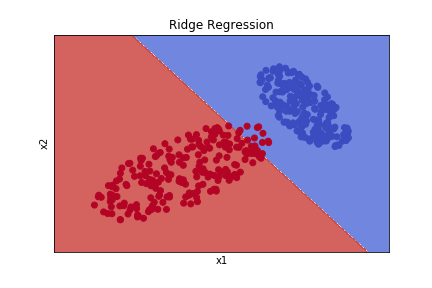
\includegraphics[scale=0.6]{1b_plot_ridge.png}
\end{figure}
\noindent

Plot of logistic regression decision boundary:
\noindent
\begin{figure}[H]
\centering
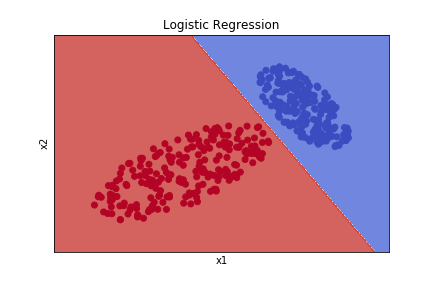
\includegraphics[scale=0.6]{1b_plot_logistic.png}
\end{figure}
\noindent

The decision boundary for the logistic regression completely separates the points according to their classifications, while the decision boundary for the ridge regression does not (it passes within the space of red points (+1 classification) points). The reason why the ridge regression does not separate the points in the dataset is because the hinge loss function only penalizes for incorrect classifications, but does not penalize for weight vectors for classifications that are very close to the classification threshold but are still correct. This results in a decision boundary that classifies data slightly worse than the logistic regression, which penalizes for weights that give correct classifications but are still too close to the classification threshold.

\problem[9] % Include the bias term x0 = 1 for all the points in S.
Leaving squared loss behind, let's focus on log loss and hinge loss. Consider the set of points $S = \{(\frac{1}{2}, 3), (2, -2), (-3, 1)\}$ in 2D space, shown below, with labels $(1, 1, -1)$ respectively.

Given a linear model with weights $w_0 = 0, w_1 = 1, w_2 = 0$ (where $w_0$ corresponds to the bias term), compute the gradients $\nabla_{w}L_{\text{hinge}}$ and $\nabla_{w}L_{\text{log}}$ of the hinge loss and log loss, and calculate their values for each point in S.

\begin{center}
  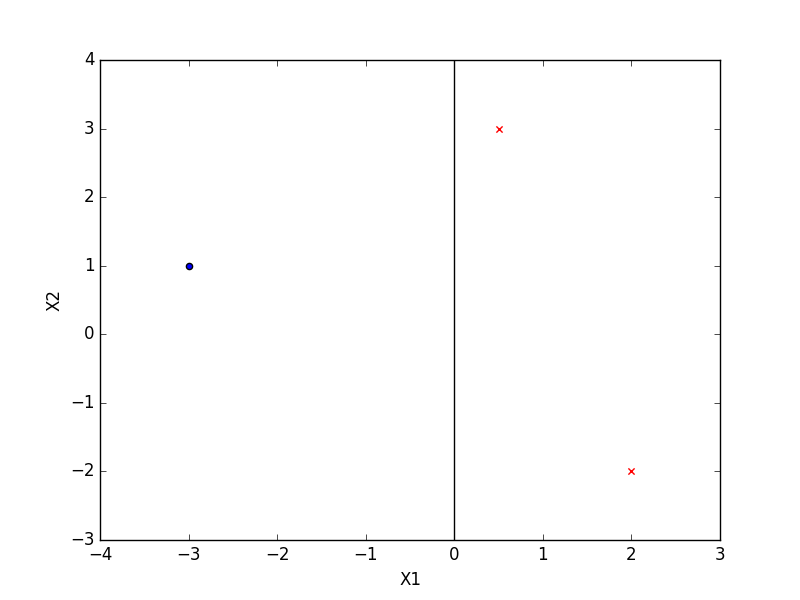
\includegraphics[width=.8\textwidth]{SimpleDatasetWithDecisionBoundary.png}
\end{center}
\begin{small}
  The example dataset and decision boundary described above. Positive instances are
  represented by red x's, while negative instances appear as blue dots.
\end{small}

For a linear model, the hinge loss function is given by $L_{\text{hinge}}(\x, y \vert \w) = \max(0, 1 - y \w^T \x)$.\\
\\
Therefore, the gradient of the hinge loss function for the linear model is
%\[ \nabla_{w}L_{\text{hinge}}(x, y \vert w) = \nabla_{w} \max(0, 1 - y w^T x) = \max(\nabla_{w} 0, \nabla_{w}(1 - y w^T x)) = \max(0, - y x)). \]
\[ \nabla_{w}L_{\text{hinge}}(\x, y \vert \w) = \nabla_{\w} \max(0, 1 - y \w^T \x) =
\begin{cases} 
   \nabla_{\w} 0 & L_{\text{hinge}}(\x, y \vert \w) \leq 0 \\
   \nabla_{\w}(1 - y \w^T \x)) & L_{\text{hinge}}(\x, y \vert \w) > 0
\end{cases} \]
\[ =
\begin{cases} 
   0 & L_{\text{hinge}}(\x, y \vert \w) = 0 \\
   - y \x & L_{\text{hinge}}(\x, y \vert \w) > 0
\end{cases}. \]

For the points in $S = \{(\frac{1}{2}, 3), (2, -2), (-3, 1)\}$ (with $S = \{(1, \frac{1}{2}, 3), (1, 2, -2), (1, -3, 1)\}$ including the $x_0$ bias terms) with labels $(1, 1, -1)$ respectively, their loss function values are $\frac{1}{2}$, $0$, and $0$ respectively. Since the point $(\frac{1}{2}, 3)$ has a positive loss function value, the gradient of this point is $- y \x = (-1, -\frac{1}{2}, -3)$. Since the last two points have loss function values of 0, the gradient values for both these points ($(2, -2)$ and $(-3, 1)$) are 0.\\
\\
For a linear model, the logistic loss function is given by\\
$L_{\text{log}}(\x, y \vert \w) = -\ln\Big(\dfrac{e^{\frac{1}{2}y f(\x \vert \w)}}{e^{\frac{1}{2}y f(\x \vert \w)} + e^{-\frac{1}{2}y f(\x \vert \w)}}\Big) = -\ln\Big(\dfrac{e^{\frac{1}{2}y \w^T \x}}{e^{\frac{1}{2}y \w^T \x} + e^{-\frac{1}{2}y \w^T \x}}\Big)$.\\
\\
Therefore, the gradient of the logistic loss function for the linear model is
\[ \nabla_{\w}L_{\text{log}}(\x, y \vert \w) = \nabla_{\w} \Big(-\ln\Big(\dfrac{e^{\frac{1}{2}y \w^T \x}}{e^{\frac{1}{2}y \w^T \x} + e^{-\frac{1}{2}y \w^T \x}}\Big)\Big) = -\dfrac{e^{\frac{1}{2}y \w^T \x} + e^{-\frac{1}{2}y \w^T \x}}{e^{\frac{1}{2}y \w^T \x}} \nabla_{\w} \Big(\dfrac{e^{\frac{1}{2}y \w^T \x}}{e^{\frac{1}{2}y \w^T \x} + e^{-\frac{1}{2}y \w^T \x}}\Big) \]
\[ = -\dfrac{e^{\frac{1}{2}y \w^T x} + e^{-\frac{1}{2}y \w^T \x}}{e^{\frac{1}{2}y \w^T \x}} \dfrac{({e^{\frac{1}{2}y \w^T \x} + e^{-\frac{1}{2}y \w^T \x}}) \nabla_{\w} {e^{\frac{1}{2}y \w^T \x}} - {e^{\frac{1}{2}y \w^T \x}} \nabla_{\w}({e^{\frac{1}{2}y \w^T \x} + e^{-\frac{1}{2}y \w^T \x}})}{({e^{\frac{1}{2}y \w^T \x} + e^{-\frac{1}{2}y \w^T \x}})^2} \]
\[ = -\dfrac{e^{\frac{1}{2}y \w^T \x} + e^{-\frac{1}{2}y \w^T \x}}{e^{\frac{1}{2}y \w^T \x}} \dfrac{({e^{\frac{1}{2}y \w^T \x} + e^{-\frac{1}{2}y \w^T \x}}) (\frac{1}{2} y \x){e^{\frac{1}{2}y \w^T \x}} - {e^{\frac{1}{2}y \w^T \x}} (\frac{1}{2} y \x)({e^{\frac{1}{2}y \w^T \x} - e^{-\frac{1}{2}y \w^T \x}})}{({e^{\frac{1}{2}y \w^T \x} + e^{-\frac{1}{2}y \w^T \x}})^2}. \]
For the points in $S = \{(\frac{1}{2}, 3), (2, -2), (-3, 1)\}$ (with $S = \{(1, \frac{1}{2}, 3), (1, 2, -2), (1, -3, 1)\}$ including the $x_0$ bias terms) with labels $(1, 1, -1)$ respectively (and with weights $w_0 = 0, w_1 = 1, w_2 = 0$), their gradient values are $(-0.377541, -0.18877, -1.13262)$, $(-0.119203, -0.238406, 0.238406)$, and $(-0.952574, 2.85772, -0.952574)$ respectively.

\problem[4]
Compare the gradients resulting from log loss to those resulting from hinge loss. When (if ever) will these gradients converge to 0? For a linearly separable dataset, is there any way to reduce or altogether eliminate training error without changing the decision boundary?

While the gradients of log loss above are all nonzero, two of the three hinge loss gradients are zero. Additionally, the nonzero gradient of hinge loss above $(-1, -\frac{1}{2}, -3)$ has a larger magnitude than any of the three logistic loss gradients above.\\
\\
For the nonzero gradient in hinge loss above ($(-1, -\frac{1}{2}, -3)$), that gradient will converge to zero once $\y\w\T\x > 1$, since then the hinge loss will become 0 and the gradient will be 0 as well.\\
\\
The gradients of logistic loss will converge to zero as the term $y \w \T \x$ increases. This is because the denominator of the gradient of the logistic loss function is $e^{\frac{1}{2} y \w \T \x}(e^{\frac{1}{2} y \w \T \x} + e^{-\frac{1}{2} y \w \T \x})^2$, so as this denominator increases, the gradients of logistic loss will converge to zero.\\
\\
For a linearly separable dataset, it is possible to reduce or altogether eliminate training error without changing the decision boundary, by changing the magnitude of the weight vector used by a machine learning model to linearly separate data based on their classifications.

\problem[5]
Based on your answer to the previous question, explain why for an SVM to be a ``maximum margin'' classifier, its learning objective must not be to minimize just $L_\text{hinge}$, but to minimize $L_\text{hinge} + \lambda\Vert w \Vert^2$ for some $\lambda > 0$.

(You don't need to prove that minimizing $L_\text{hinge} + \lambda\Vert w \Vert^2$ results in a maximum margin classifier; just show that the additional penalty term addresses the issues of minimizing just $L_\text{hinge}$.)

By minimizing the $\lambda \vv{w}^2$ term in the SVM learning objective, this minimizes the term $\vv{w}^2$, which is equivalent to maximizing $1/\vv{w}^2$. Since $1/\vv{w}^2$ is maximizing the margin with a linear separating model, this explains why for an SVM to be a ``maximum margin'' classifier, its learning objective must not be to minimize just $L_\text{hinge}$, but to minimize $L_\text{hinge} + \lambda\Vert w \Vert^2$ for some $\lambda > 0$.

% problem 2
\newpage
\section{Effects of Regularization}
\textit{Relevant materials: Lecture  4}

For this problem, you are required to implement everything yourself and submit code.
\indent\problem[4] % indent for consistency
In order to prevent over-fitting in the least-squares linear regression problem, we add a regularization penalty term.
Can adding the penalty term decrease the training (in-sample) error?
Will adding a penalty term always decrease the out-of-sample errors?
Please justify your answers. Think about the case when there is over-fitting while training the model.

Adding the penalty term cannot decrease the training (in-sample) error, because the regularization term adds an augmented error to the loss function, making the training error greater than or equal to what the training error would be without regularization.\\
\\
Adding a penalty term will not always decrease the out-of-sample errors. When over-fitting to the training model without regularization, adding an optimal regularization term penalty will decrease the out-of-sample errors. However, adding an non-optimal regularization term penalty (with $lambda$ too small or too large) will not decrease the out-of-sample errors.

\problem[4]
$\ell_1$ regularization is sometimes favored over $\ell_2$ regularization due to its ability to generate a sparse $w$ (more zero weights).
In fact, $\ell_0$ regularization (using $\ell_0$ norm instead of $\ell_1$ or $\ell_2$ norm) can generate an even sparser $w$, which seems favorable in high-dimensional problems.
However, it is rarely used.  Why?

$\ell_0$ regularization is rarely used because $\ell_0$ regularization loss function is not continuous (the function is flat and discontinuous), making it very difficult to optimize over.

\subsection{Implementation of \texorpdfstring{$\ell_2$}{L2} regularization:}

We are going to experiment with regression for the Red Wine Quality Rating data set. The data set is uploaded on the course website, and you can read more about it here: \url{https://archive.ics.uci.edu/ml/datasets/Wine}. The data relates 13 different factors (last 13 columns) to wine type (the first column). Each column of data represents a different factor, and they are all continuous features. Note that the original data set has three classes, but one was removed to make this a binary classification problem.

Download the data for training and testing.
There are two training sets, wine\_training1.txt (100 data points) and wine\_training2.txt (a proper subset of wine\_training1.txt containing only 40 data points), and one test set, wine\_testing.txt (30 data points). You will use the wine\_testing.txt dataset to evaluate your models.

We will train a \emph{$\ell_2$-regularized logistic regression} model on this data. Recall that the unregularized logistic error (a.k.a. log loss) is
\[E = -\sum_{i=1}^{N}\log(p(y_i | \mathbf{x}_i))\]

where $p(y_i = -1 | \mathbf{x}_i)$ is
\[\frac{1}{1 + e^{\mathbf{w}^T\mathbf{x}_i}}\]

and $p(y_i = 1 | \mathbf{x}_i)$ is
\[\frac{1}{1 + e^{-\mathbf{w}^T\mathbf{x}_i}},\]
where as usual we assume that all $\mathbf{x}_i$ contain a bias term.
The $\ell_2$-regularized logistic error is
\begin{align*}
  E &= -\sum_{i=1}^{N}\log(p(y_i | \mathbf{x}_i)) + \lambda\mathbf{w}^T\mathbf{w} \\
    &= -\sum_{i=1}^{N} \log \left( \frac{1}{1 + e^{-y_i\mathbf{w}^T\mathbf{x}_i}} \right) + \lambda\mathbf{w}^T\mathbf{w} \\
    &= -\sum_{i=1}^{N} \left(\log \left( \frac{1}{1 + e^{-y_i\mathbf{w}^T\mathbf{x}_i}} \right) - \frac{\lambda}{N}\mathbf{w}^T\mathbf{w}\right).
\end{align*}
Implement SGD to train a model that minimizes the $\ell_2$-regularized logistic error, i.e. train an $\ell_2$-regularized logistic regression model.  Train the model with 15 different values of $\lambda$ starting with $\lambda_0 = 0.00001$ and increasing by a factor of 5, i.e. $$\lambda_0 = 0.00001, \lambda_1 = 0.00005, \lambda_2 = 0.00025, ..., \lambda_{14} = 61,035.15625.$$
\par

Some important notes: Terminate the SGD process after 20,000 epochs, where each epoch performs one SGD iteration for each point in the training dataset. You should shuffle the order of the points before each epoch such that you go through the points in a random order (hint: use \texttt{numpy.random.permutation}). Use a learning rate of $5e-4$, and initialize your weights to small random numbers.

You may run into numerical instability issues (overflow or underflow). One way to deal with these issues is by normalizing the input data $X$. Given the column for the $j$th feature, $X_{:,j}$, you can normalize it by setting $X_{ij} = \frac{X_{ij} - \overline{X_{:,j}} }{\sigma(X_{:,j})}$ where $\sigma(X_{:,j})$ is the standard deviation of the $j$th column's entries, and $\overline{X_{:,j}}$ is the mean of the $j$th column's entries. Normalization may change the optimal choice of $\lambda$; the $\lambda$ range given above corresponds to data that has been normalized in this manner. If you treat the input data differently, simply plot enough choices of $\lambda$ to see any trends.

\problem[16]
Do the following for both training data sets (wine\_training1.txt and wine\_training2.txt) and attach your plots in the homework submission (use a log-scale on the horizontal axis):

\subproblem Plot the average training error ($E_\text{in}$) versus different $\lambda$s.

\subproblem Plot the average test error ($E_\text{out}$) versus different $\lambda$s using wine\_testing.txt as the test set.

\subproblem Plot the $\ell_2$ norm of $\mathbf{w}$ versus different $\lambda$s. \medskip

 You should end up with three plots, with two series (one for wine\_training1.txt and one for wine\_training2.txt) on each plot. Note that the $E_\text{in}$ and $E_\text{out}$ values you plot should not include the regularization penalty --- the penalty is only included when performing gradient descent.

Plot of the average training error ($E_\text{in}$) versus different $\lambda$s:
\noindent
\begin{figure}[H]
\centering
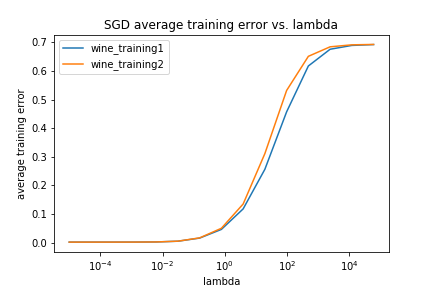
\includegraphics[scale=0.6]{2c_plot_train_errors.png}
\end{figure}
\noindent
Plot of the average test error ($E_\text{out}$) versus different $\lambda$s:
\noindent
\begin{figure}[H]
\centering
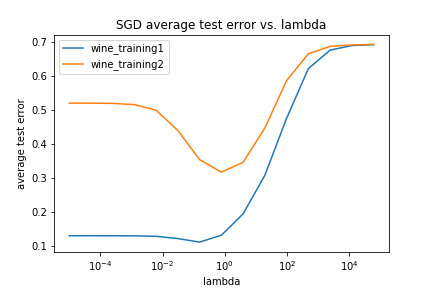
\includegraphics[scale=0.6]{2c_plot_test_errors.png}
\end{figure}
\noindent
Plot of the $\ell_2$ norm of $\mathbf{w}$ versus different $\lambda$s:
\noindent
\begin{figure}[H]
\centering
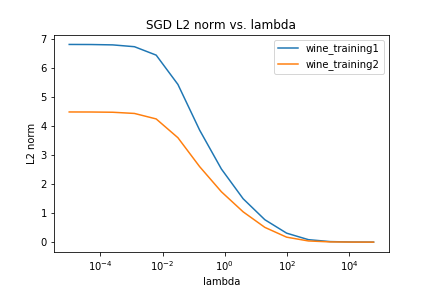
\includegraphics[scale=0.6]{2c_plot_l2_norms.png}
\end{figure}
\noindent

\problem[4]
Given that the data in wine\_training2.txt is a subset of the data in wine\_training1.txt, compare errors (training and test) resulting from training with wine\_training1.txt (100 data points) versus wine\_training2.txt (40 data points). Briefly explain the differences.

For the wine\_training1.txt and wine\_training2.txt training errors, over all $\lambda$s, the training errors are very close if not about equal to each other. This is because SGD is able to find near-zero error with both training sets, and for large $\lambda$s, the regularization term in the SGD gradient dominates the behavior of SGD resulting in similar training errors between the two datasets for large $\lambda$s ($\lambda \geq 1$).\\
\\
For the wine\_training1.txt and wine\_training2.txt test errors, for $\lambda < 1000$, wine\_training2.txt has higher test errors than wine\_training1.txt. This is because wine\_training2.txt contains less data than wine\_training1.txt, resulting in SGD overfitting to the limited data in wine\_training2.txt.

\problem[4]
Briefly explain the qualitative behavior (i.e. over-fitting and under-fitting) of the training and test errors with different $\lambda$s while training with data in wine\_training1.txt.

For training errors (with the dataset wine\_training1.txt) corresponding to large $\lambda$s, under-fitting occurs, because as $\lambda$ increases, the bias of the model increases, causing the training and test errors for large $\lambda$s to increase as well. For $\lambda < 0.15625 = \lambda_6$, slight over-fitting occurs, because while training error for wine\_training1.txt for these $\lambda$ values is very close to zero, test errors for these $\lambda$ values are slightly higher than that of $\lambda = 0.15625$.

\problem[4]
Briefly explain the qualitative behavior of the $\ell_2$ norm of $\textbf{w}$ with different $\lambda$s while training with the data in wine\_training1.txt.

The $\ell_2$ norm of $\textbf{w}$ while training with the data in wine\_training1.txt is constant for small $\lambda$s ($\lambda < 0.001$), then the $\ell_2$ norm of $\textbf{w}$ decreases exponentially for increasing $\lambda$ for $\lambda >= 0.001$.

\problem[4]
If the model were trained with wine\_training2.txt, which $\lambda$ would you choose to train your final model? Why?

If the model were trained with wine\_training2.txt, $\lambda = \lambda_7 = 0.78125$ would be choosen to train the final model because this value of lambda results in the model having the minimum test error when trained with the wine\_training2.txt dataset.

% Question 3
\newpage
\section{Lasso (\texorpdfstring{$\ell_1$}{L1}) vs. Ridge (\texorpdfstring{$\ell_2$}{L2}) Regularization}
\textit{Relevant materials: Lecture 3}

For this problem, you may use the scikit-learn (or other Python package) implementation of Lasso and Ridge regression --- you don't have to code it yourself.

The two most commonly-used regularized regression models are Lasso ($\ell_1$) regression and Ridge ($\ell_2$) regression.
Although both enforce ``simplicity'' in the models they learn, only Lasso regression results in sparse weight vectors.
This problem compares the effect of the two methods on the learned model parameters.

\problem[12] % Specific problem (linear regresion - P(w|D) gaussion), run lasso and ridge, and plot parameters vs lambda (linear scale for lambda is more interpretable)
The tab-delimited file problem3data.txt on the course website contains 1000 9-dimensional datapoints.  The first 9 columns contain $x_1,\ldots,x_9$, and the last column contains the target value $y$.

\subproblem
Train a linear regression model on the problem3data.txt data with Lasso regularization for regularization strengths $\alpha$ in the vector given by \texttt{numpy.linspace(0.01, 3, 30)}.
On a single plot, plot each of the model weights $w_1, ..., w_9$ (ignore the bias/intercept) as a function of $\alpha$.

Plot of each of the model weights $w_1, ..., w_9$ as a function of $\alpha$ (with Lasso regression):
\noindent
\begin{figure}[H]
\centering
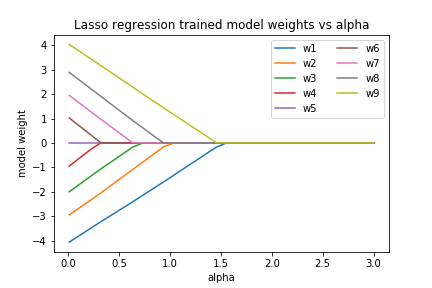
\includegraphics[scale=0.6]{3a_plot_lasso.png}
\end{figure}
\noindent

\subproblem
Repeat \textbf{i.} with Ridge regression, and this time using regularization strengths $\alpha \in \{1, 2, 3, \ldots, 1e4\}$.

Plot of each of the model weights $w_1, ..., w_9$ as a function of $\alpha$ (with Ridge regression):
\noindent
\begin{figure}[H]
\centering
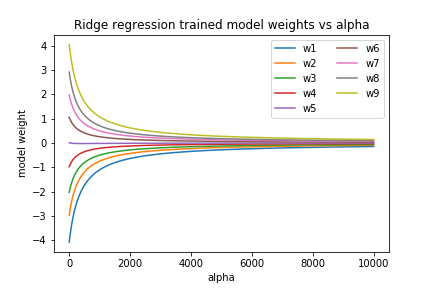
\includegraphics[scale=0.6]{3a_plot_ridge.png}
\end{figure}
\noindent

\subproblem
As the regularization parameter increases, what happens to the number of model weights that are exactly zero with Lasso regression?
What happens to the number of model weights that are exactly zero with Ridge regression?

As the regularization parameter increases, the number of model weights that are exactly zero increases with Lasso regression.\\
\\
As the regularization parameter increases, the number of model weights that are exactly zero mostly stays constant with Ridge regression ($w_5$ starts out nonzero at $\alpha = 0$ and then becomes 0 before $\alpha = 1000$, but this is the only weight that becomes 0 for Ridge regression, although all the model weights approach zero as $\alpha$ increases).

\medskip
\lstset{
  basicstyle=\small\ttfamily,
  breaklines=true,
  columns=fullflexible
}



\problem[18]

\subproblem
In the case of 1-dimensional data, Lasso regression admits a closed-form solution.
Given a dataset containing $N$ datapoints each with $d$ features, where $d = 1$, solve for
\[\underset{w}{\argmin} \Vert\mathbf{y} - \mathbf{x}w\Vert^2 + \lambda\Vert w\Vert_1,
\]
where $\mathbf{x} \in \mathbb{R}^{N}$ is the vector of datapoints and $\mathbf{y} \in \mathbb{R}^N$ is the  vector of all output values corresponding to these datapoints. Just consider the case where $d = 1$, $\lambda \geq 0$, and the weight $w$ is a scalar.

This is linear regression with Lasso regularization.

To solve for $\underset{w}{\argmin} \Vert\mathbf{y} - \mathbf{x}w\Vert^2 + \lambda\Vert w\Vert_1$, set the derivative of the expression $\Vert\mathbf{y} - \mathbf{x}w\Vert^2 + \lambda\Vert w\Vert_1$ with respect to $w$ equal to 0, since the minimum value of the given expression is at a location such that the derivative at the location with respect to $w$ is 0.
\[ \Vert\y - \x w\Vert^2 + \lambda\Vert w\Vert_1 = (\y - \x w)\T(\y - \x w) + \lambda\Vert w\Vert_1 = (\y\T - \x\T w)(\y - \x w) + \lambda\Vert w\Vert_1 \]
\[ \y\T\y - \y\T\x w - \x\T w \y + \x\T\x w^2 + \lambda\Vert w\Vert_1. \]
Therefore,
\[ \frac{\partial}{\partial w}(\Vert\y - \x w\Vert^2 + \lambda\Vert w\Vert_1) = 0 \implies \frac{\partial}{\partial w}(\y\T\y - \y\T\x w - \x\T w \y + \x\T\x w^2 + \lambda\Vert w\Vert_1) = 0 \]
\[ \implies 0 - \y\T\x - \x\T\y + 2\x\T\x w + \lambda\sign(w) = 0. \]
Since $\y\T\x = \x\T\y$,
\[ 0 - \y\T\x - \x\T\y + 2\x\T\x w + \lambda\sign(w) = 0 \implies -2\y\T\x + 2\x\T\x w + \lambda\sign(w) = 0 \implies 2\x\T\x w = 2\y\T\x - \lambda\sign(w) \]
\[ \implies w = \dfrac{2\y\T\x - \lambda\sign(w)}{2\x\T\x}, \]
where
\[ \sign(w) =
\begin{cases} 
   -1 & w < 0 \\
   1 & w > 0 \\
   [-1, 1] & w = 0
\end{cases}. \]

\subproblem
In this question, we continue to consider Lasso regularization in 1-dimension. Now, suppose that when $\lambda = 0$, $w \neq 0$. Does there exist a value for $\lambda$ such that $w = 0$? If so, what is the smallest such value?

Using the expression for $w$ obtained in part i and setting $w > 0$,
\[ w = \dfrac{2\y\T\x - \lambda(1)}{2\x\T\x} \implies w = \dfrac{2\y\T\x - \lambda}{2\x\T\x}. \]
Since $w > 0$ and $\x\T\x > 0$, $2\y\T\x - \lambda > 0 \implies 2\y\T\x > \lambda$.\\
\\
Using the expression for $w$ obtained in part i and setting $w < 0$,
\[ w = \dfrac{2\y\T\x - \lambda(-1)}{2\x\T\x} \implies w = \dfrac{2\y\T\x + \lambda}{2\x\T\x}. \]
Since $w < 0$ and $\x\T\x > 0$, $2\y\T\x + \lambda > 0 \implies 2\y\T\x < -\lambda$.\\
\\
Since $2\y\T\x > \lambda$ for $w > 0$ and $2\y\T\x < -\lambda$ for $w < 0$, for $w = 0$, $-\lambda \leq 2\y\T\x \leq \lambda \implies \lambda \geq 2\vert \y\T\x \vert$. Therefore, the smallest value of $\lambda$ such that $w = 0$ is $\lambda = 2\vert \y\T\x \vert$.

\subproblem
Given a dataset containing $N$ datapoints each with $d$ features, solve for
\[\underset{\mathbf{w}}{\argmin} \Vert\mathbf{y} - \mathbf{X}\mathbf{w}\Vert^2 + \lambda\Vert\mathbf{w}\Vert_2^2
\]
where $\mathbf{X} \in \mathbb{R}^{N \times d}$ is the matrix of datapoints and $\mathbf{y} \in \mathbb{R}^N$ is the  vector of all output values for these datapoints. Do so for arbitrary $d$ and $\lambda \geq 0$.

This is linear regression with Ridge regularization.

To solve for $\underset{\w}{\argmin} \Vert \y - \X \w \Vert^2 + \lambda\Vert \w\Vert_2^2$, set the derivative of the expression $\Vert \y - \X \w \Vert^2 + \lambda\Vert \w\Vert_2^2$ with respect to $\w$ equal to 0, since the minimum value of the given expression is at a location such that the derivative at the location with respect to $\w$ is 0.
\[ \Vert \y - \X \w \Vert^2 + \lambda\Vert \w\Vert_2^2 = (\y - \X \w)\T(\y - \X \w) + \lambda \w\T\w = (\y\T - \w\T\X\T)(\y - \X \w) + \lambda \w\T\w \]
\[ \y\T\y - \y\T \X\w - \w\T\X\T \y + \w\T\X\T \X\w + \lambda \w\T\w. \]
Using the matrix derivative rules $\frac{\partial}{\partial \w}(\w\T \va) = \frac{\partial}{\partial \w}(\va\T \w) = \va$ and $\frac{\partial}{\partial \w}(\w\T\A\w) = \A\T\w + \A\w = (\A\T + \A)\w$,
\[ \frac{\partial}{\partial \w}(\Vert \y - \X \w \Vert^2 + \lambda\Vert \w\Vert_2^2) = 0 \implies \frac{\partial}{\partial \w}(\y\T\y - \y\T \X\w - \w\T\X\T \y + \w\T\X\T \X\w + \lambda \w\T\w) = 0 \]
\[ \implies 0 - \X\T\y - \X\T\y + 2 \X\T\X\w + 2\lambda \w = 0 \implies \X\T\X\w + \lambda\w = \X\T\y \implies (\X\T\X + \lambda I)\w = \X\T\y, \]
where $I$ is the identity matrix (with dimensions equal to those of $\X\T\X$). By the invertible matrix theorem, $(\X\T\X + \lambda I)^{-1}$ exists. Therefore, $\w = (\X\T\X + \lambda I)^{-1}\X\T\y$.

\subproblem In this question, we consider Ridge regularization in 1-dimension. Suppose that when $\lambda = 0$, $w \neq 0$. Does there exist a value for $\lambda > 0$ such that $w = 0$? If so, what is the smallest such value?

From part iii, in 1-dimension, $w = (\X\T\X + \lambda I)^{-1}\X\T\y$. Given that when $\lambda = 0$, $w \neq 0$,\\
$w = (\X\T\X + (0) I)^{-1}\X\T\y = (\X\T\X)^{-1}\X\T\y$. By the invertible matrix theorem, $(\X\T\X)^{-1}$ has an inverse, so $(\X\T\X)^{-1}$ is a nonzero matrix. Since $w$ is nonzero and $(\X\T\X)^{-1}$ is nonzero in $w = (\X\T\X)^{-1}\X\T\y$, $\X\T\y$ must also be nonzero. For $\lambda > 0$, by the invertible matrix theorem, $(\X\T\X + \lambda I)^{-1}$ has an inverse, so $(\X\T\X + \lambda I)^{-1}$ must be nonzero, and since $\X\T\y$ is also nonzero, $w = (\X\T\X + \lambda I)^{-1}\X\T\y$ must also be nonzero for all $\lambda > 0$. Therefore, there does not exist a value for $\lambda > 0$ such that $w = 0$.

\end{document}

%%% Local Variables:
%%% mode: latex
%%% TeX-master: t
%%% End:
